\AuthorInfo{
name=,
headings=\textsc{Luca De Feo},
institution={IBM Research GmbH},
address={Säumerstrasse 4, Rüschlikon, Schweiz},
email={aracne-2021@defeo.lu},
} %da inserire all'inizio del contributo


\chapter[toc=Demystifying Isogeny Based Cryptography\\{\protect\small\emph{Luca De Feo}}, headings=Isogeny Based Cryptography]{Demystifying Isogeny Based Cryptography\\\vspace{2mm}\normalsize \textsc{Luca De Feo}\protect}

\addtocontents{toc}{\protect\vspace{-4mm}}

\begin{otherlanguage}{english}
  \def\Z{\mathbb{Z}}
  \def\F{\mathbb{F}}
  \def\exp{\mathrm{exp}}
  \def\com{\mathcal{C}}
  \def\Gal{\mathrm{Gal}}
  \def\End{\mathrm{End}}
  \def\O{\mathcal{O}}
  
  Isogenies, what are they? Like the character in Alessandro Manzoni's
  novel, cryptographers encountering an isogeny in a textbook would
  have been justified, ten years ago, asking themselves ``\textit{chi
    era costui?}''\footnote{``Who was he?'', inquires Don Abbondio
    upon reading the name of Carneades in a hagiography of St Charles
    Borromeo.} Elliptic curves, that, we know. But isogenies?  The
  name sounds familiar, it must be one of those math things starting
  in iso-; but \textit{chi diavolo era costui?}\footnote{There would
    be much to say about how Manzoni's \textit{faux savant}
    characters, from Don Abbondio to Don Ferrante, speak of our
    time. But this is an article about isogenies.}

  That is no longer true. Any self-respecting cryptographer nowadays
  must have at least a vague idea of what isogenies are and how they
  are used in cryptography. This survey is your guide to the
  supersingular isogeny galaxy~\cite{galaxy}.

  \section{\textit{Aufstieg und Fall der Elliptische Kurven Kryptografie}}
  Elliptic curves are today a fact of life.  I sometimes wonder what
  Euler would have thought of it.  Not a single day goes without
  billions of elliptic curve operations being performed by servers,
  laptops, smartphones and even refrigerators throughout the world. I
  suppose Euler would have loved the fridge.

  Why are elliptic curves so important in cryptography? One reason is
  that they are the closest thing we know to a \emph{generic
    group}. What cryptographers ask from a group is: to be abelian, to
  be finite, to have efficient algorithms for testing membership,
  equality, and for evaluating the group operation. Any group well
  mannered enough to do exactly what is asked from it, and nothing
  more, is called \emph{generic}.

  The most important operation for a cryptographic group is
  \emph{exponentiation}:
  \begin{align*}
    \exp_g : \Z &\to G,\\
    x &\mapsto g^x.
  \end{align*}
  That $\exp_g(n)$ can be evaluated using $O(\log(n))$ generic group
  operations is obvious. What makes a group precious is the inverse
  map $g^x\mapsto x$, the \emph{discrete logarithm}, being
  ``difficult'' to compute. Then $\exp_g$ is what cryptographers call
  a \emph{one-way function}.

  The other reason they are loved, and I claim it is the most
  important one, is that no knowledge of elliptic curves is required
  in order to make cryptography out of them.  Cryptography is like
  humanity in Plato's cave: it only sees the tame generic group shadow
  of a wild real world elliptic curve. Do not get me wrong: this is
  great! We wouldn't have as powerful cryptographic tools, if creating
  them required a deep knowledge in number theory. We do not have such
  a luxury with isogenies.
  
  What can you do with a generic group? A lot of things. I am sure the
  reader is familiar with the Diffie--Hellman key
  exchange~\cite{DifHel76}, but I want to highlight a different
  application. A \emph{commitment scheme} is the cryptographic
  equivalent of a sealed envelope: in the first phase a party
  \emph{commits to} a message $m$ (\emph{e.g.}, a monetary offering)
  by publishing a \emph{commitment} $\com(m;r)$, where $r$ represents
  an arbitrary auxiliary input (typically, some random bits); in the
  second phase, the party \emph{opens} the commitment by revealing $m$
  and $r$; anyone can check that $m$ is the message originally
  committed to by recomputing $\com(m;r)$.  A cryptographic commitment
  must satisfy two properties: it must be \emph{binding}, \emph{i.e.},
  after having committed to $\com(m;r)$ it must be difficult for the
  party to find $(m',r')$ with $m\ne m'$ such that
  $\com(m';r')=\com(m;r)$; and it must by \emph{hiding}, \emph{i.e.},
  given only $\com(m;r)$ it must be difficult to deduct $m$.

  Given a generic group $G$ with some fixed generator $g$, it is easy
  to imagine a simple commitment scheme defined by $\com(m) =
  g^m$. This scheme is obviously binding if $0<m<\#G$, and is hiding
  thanks to the one-wayness of the $\exp_g$ function. However, while
  the binding property is \emph{perfect} (it's impossible for the
  party to cheat), the hiding property only holds against
  \emph{computationally bounded} adversaries, rather than in an
  information-theoretic sense. This may be a problem if, for example,
  the messages $m$ are likely to be taken from a small subset.

  Pedersen~\cite{C:Pedersen91} is credited with a very simple and
  elegant idea to obtain a perfectly hiding commitment scheme from
  generic groups. Let $g$ and $h$ be two random generators of $G$, he
  defined $\com(m;r)=g^m h^r$, where $r$ is a random integer in
  $[1,\#G]$. It is easy to see that Pedersen's commitment is perfectly
  hiding, thanks to $h^r$ being uniformly distributed in $G$. For the
  binding property, it is capital that the discrete logarithm relation
  between $g$ and $h$ is unknown to the committer; indeed, given
  $x=\log_g(h)$ the commitment simply becomes $g^{m+xr}$, and breaking
  binding simply amounts to solving the equation $m+xr=m'+xr'$ modulo
  $\#G$.

  Pedersen commitments can do much more than just emulate digital
  envelopes, and in fact a great variety of cryptographic protocols is
  based on them and similar ideas. Most of the advanced cryptographic
  protocols used nowadays, such as the Signal protocol used by
  WhatsApp, or those used in privacy-preserving cryptocurrencies, use
  some advanced features of generic groups such as Pedersen
  commitments; and their generic group of choice is, inevitably,
  elliptic curves.

  But the reader knows the story by now: our world is coming to an
  end, Shor's bane is free~\cite{FOCS:Shor94}, soon hordes of quantum
  computers will roam the earth, mercilessly hunting down discrete
  logarithms and composite integers, our mobile data plans will
  evaporate in just days to accommodate for post-quantum cryptography.

  \section{Isogeny graphs}
  I will assume some familiarity with elliptic curves and abstract
  algebra. At this point, we're obliged to chose a camp in a
  controversy as ancient as ``Emacs vs vi'': unlike cryptographers,
  algebraists like to write abelian groups additively. We will side
  with the algebraists and rewrite exponentiation as
  \[[n]P \equiv \exp_P(n),\] with the side-effect of loosing track of
  the original meaning of ``discrete logarithm''.

  The \emph{multiplication map} $[n]$ is an example of a morphism from
  an elliptic curve to itself.  Isogenies are generalizations of these
  morphisms, when we view elliptic curves both as groups and as
  algebraic varieties.

  \begin{definition}
    Let $\varphi:E\to E'$ be a map between two elliptic curves defined
    over an algebraically closed field, the following are equivalent:
    \begin{enumerate}
    \item $\varphi$ is a surjective group morphism,
    \item $\varphi$ is a group morphism with finite kernel,
    \item $\varphi$ is a non-constant algebraic map of projective
      varieties sending the point at infinity of $E$ onto the point at
      infinity of $E'$.
    \end{enumerate}
    In any of these cases, $\varphi$ is called an \emph{isogeny}; or
    an \emph{endomorphism} when $E=E'$.
  \end{definition}

  In cryptography, however, we typically deal with non-algebraically
  closed fields. In this case we need to take \emph{rationality} into
  account. Let $k$ be a field with algebraic closure $\bar{k}$. By
  $E/k$ we mean a curve defined over $k$, \emph{i.e.}, whose equation
  has coefficients in $k$. We can extend scalars to $\bar{k}$, and see
  $E$ as a curve over $\bar{k}$; when it is necessary to distinguish
  between them, we will write $E(\bar{k})$ for the group of points in
  the algebraic closure, and $E(k)$ for the group of
  \emph{$k$-rational} points.  Then the Galois group of $\bar{k}/k$
  acts on $E(\bar{k})$ by permuting its elements.

  \begin{definition}
    Let $E$, $E'$ be elliptic curves defined over $k$. Let
    $\varphi:E\to E'$ be an isogeny. We say that $\varphi$ is
    \emph{defined over $k$}, or \emph{$k$-rational} if any of the
    following equivalent conditions holds.
    \begin{enumerate}
    \item $\sigma(\ker\varphi) = \ker\varphi$ for any
      $\sigma\in\Gal(\bar{k}/k)$,
    \item $\sigma\circ\varphi = \varphi\circ\sigma$ for any
      $\sigma\in\Gal(\bar{k}/k)$,
    \item $\varphi$ is expressed by rational fractions with
      coefficients in $k$.
    \end{enumerate}
  \end{definition}

  Note that if $\varphi$ is $k$-rational, the points in $\ker\varphi$
  are not necessarily defined over $k$. To give a complete
  introduction to isogenies we would need to define separability vs
  inseparability, degree, and more. However to keep this presentation
  light we will skip these, and direct the curious reader
  to~\cite{silverman:elliptic,milne2006,defeo2017isogenybased}.  Here,
  unless stated otherwise, all isogenies will be \emph{separable}, and
  $\deg\varphi=\#\ker\varphi$.

  \begin{theorem}[Dual isogeny theorem]
    Let $\varphi:E\to E'$ be an isogeny of degree $m$. %
    There is a unique isogeny $\hat{\varphi}:E'\to E$, called the
    \emph{dual isogeny}, such that
    \[\hat{\varphi}\circ\varphi = [m]_E, \quad \varphi\circ\hat{\varphi} = [m]_{E'}.\] %
  \end{theorem}

  \paragraph{Example.}
  The map $\varphi$ from the elliptic curve $y^2=x^3+x$ to $y^2=x^3-4x$
  defined by
  \begin{equation*}
      \varphi(x,y) = \left(\frac{x^2+1}{x},y\frac{x^2-1}{x^2}\right),\qquad
      \varphi(0,0) = \varphi(\O) = \O
  \end{equation*}
  is a separable isogeny between curves defined over $\mathbb{Q}$. %
  It has degree $2$, and its kernel is generated by the point
  $(0,0)$. %
  Its dual is defined by
  \begin{equation*}
      \hat\varphi(x,y) = \left(\frac{x^2-4}{4x},y\frac{x^2+4}{8x^2}\right),\qquad
      \hat\varphi(0,0) = \varphi(\O) = \O.
  \end{equation*}

  Isogenies have been used in cryptography since the early days of
  Elliptic Curve Cryptography, most notably within the
  Schoof--Elkies--Atkin point counting algorithm~\cite{schoof95}.  But
  there is a general agreement that Isogeny Based Cryptography starts
  from the moment one stops focusing on a single elliptic curve with
  its isogenies, and \emph{zooms out} to encompass \emph{all} elliptic
  curves with isogenies between them.

  An \emph{isogeny graph} is a multi-graph whose vertices represent
  elliptic curves, and whose edges represent isogenies. By putting
  different kinds of restrictions on the curves and the isogenies, we
  obtain different isogeny graphs with interesting properties.

  In general, it is easier to think of the vertices as
  isomorphism\footnote{An isomorphism is an isogeny of degree 1,
    \emph{i.e.}, a bijective isogeny.} classes of elliptic
  curves. Conveniently, the $j$-invariant classifies elliptic curves
  up to isomorphism (over the algebraic closure), thus we typically
  attach a single $j$-invariant to each vertex. Sometimes, a finer
  notion of isomorphism will have to be considered (\emph{e.g.},
  isomorphism over the base field $k$), and a different invariant
  corresponding to this isomorphism type will be used instead
  (\emph{e.g.}, a Montgomery $A$-invariant as used in CSIDH).
  
  For the edges, we will usually restrict to isogenies of a given
  degree, or possibly of degree taken in some small list. Hence,
  isogeny graphs will tend to be undirected (representing an isogeny
  and its dual by the same undirected edge), and regular (\emph{e.g.},
  for any prime $\ell$ different from the characteristic, any curve
  has exactly $\ell+1$ isogenies of degree $\ell$ in the algebraic
  closure).

  Figures~\ref{fig:sidh} and~\ref{fig:csidh} show two important
  examples of isogeny graphs. On the right, the graph of all
  supersingular curves defined over $\F_{89}$, up to
  $\F_{89}$-rational isomorphisms. These are the curves of
  $j$-invariant $0$, $66$, $52$, $13$, $7$ or $6$; each $j$-invariant
  being repeated twice, because each curve has a
  non-$\F_{89}$-isomorphic copy called the \emph{quadratic twist}. The
  edges are the union of three distinct edge sets (represented by
  different colors), corresponding to the $\F_{89}$-rational isogenies
  of degree $3$, $5$ and $7$, respectively.

  \begin{figure}
    \pgfkeys{/triangle/.code=\tikzset{x={(-0.5cm,-0.866cm)},y={(1cm,0cm)}}}
    \pgfkeys{/lattice/.code n args={4}{\tikzset{cm={#1,#2,#3,#4,(0,0)}}}}
    \centering
    \begin{minipage}{0.47\textwidth}
      \centering
      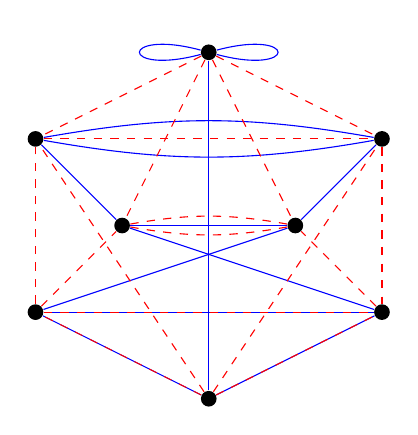
\begin{tikzpicture}[x=1.1cm,y=1.1cm]
        \begin{scope}[every node/.style={fill,black,circle,inner sep=2pt}]
          \node at (0,0)  (1){};
          \node at (0,4) (20){};
          \node at (2,1)  (16z){};
          \node at (-2,1)  (81z){};
          \node at (-1,2) (77z){};
          \node at (1,2)  (20z){};
          \node at (-2,3)  (85z){};
          \node at (2,3)  (12z){};
        \end{scope}
        
        \begin{scope}[blue,every loop/.style={looseness=50}]
          \path (1) edge (20) edge (16z) edge (81z);
          \path (20) edge[loop left] (20) edge[loop right] (20);
          \path (16z) edge (81z) edge (77z);
          \path (81z) edge (20z);
          \path (77z) edge (20z) edge (85z);
          \path (20z) edge (12z);
          \path (12z) edge[bend right=10] (85z) edge[bend left=10] (85z);
        \end{scope}
        
        \begin{scope}[red,dashed]
          \path (1) edge (85z) edge (81z) edge (12z) edge (16z);
          \path (20) edge (85z) edge (77z) edge (20z) edge (12z);
          \path (81z) edge (85z) edge (77z) edge (16z);
          \path (85z) edge (12z);
          \path (12z) edge (16z);
          \path (16z) edge (20z);
          \path (20z) edge[bend right=10] (77z) edge[bend left=10] (77z);
        \end{scope}
      \end{tikzpicture}
      \caption{The supersingular isogeny graphs of degree 2
        (blue,continuous) and 3 (red,dashed) on $\F_{97^2}$.}
      \label{fig:sidh}
    \end{minipage}
    \hfill
    \begin{minipage}{0.47\textwidth}
      \centering
      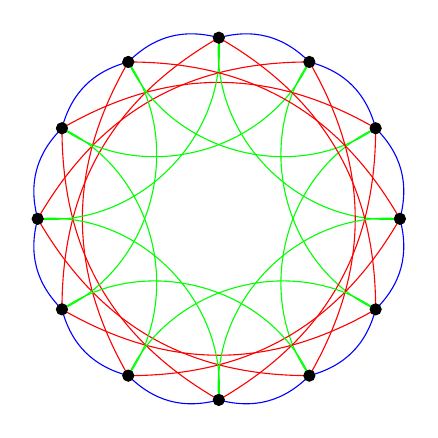
\begin{tikzpicture}
        \def\crater{12}
        \def\jumpa{-8}
        \def\jumpb{9}
        \def\diam{2.3cm}

        \foreach \i in {1,...,\crater} {
          \draw[blue] (360/\crater*\i : \diam) to[bend right] (360/\crater*\i+360/\crater : \diam);
          \draw[red] (360/\crater*\i : \diam) to[bend right] (360/\crater*\i+\jumpa*360/\crater : \diam);
          \draw[green] (360/\crater*\i : \diam) to[bend right=50] (360/\crater*\i+\jumpb*360/\crater : \diam);
        }
        \foreach \i in {1,...,\crater} {
          \pgfmathparse{int(mod(2^\i,13))}
          \let\exp\pgfmathresult
          \draw[fill] (360/\crater*\i: \diam) circle (2pt);
        }
      \end{tikzpicture}
      \caption{The supersingular isogeny graphs of degree 3 (blue), 5
        (red) and 7 (green), restricted to $\F_{89}$-rational
        isomorphism classes.\\
        Also the connected component of $j=77$ in the ordinary isogeny
        graph of $\F_{233}$ (same isogeny degrees).}
      \label{fig:csidh}
    \end{minipage}
  \end{figure}

  This graph also occurs as a connected component of infinitely many
  ordinary graphs, for example the component containing the
  $j$-invariants $20$, $28$, $40$, $77$, $86$, $87$, $118$, $136$,
  $138$, $142$, $184$ and $194$ over $\F_{233}$ ---in the ordinary
  case, the quadratic twists form a distinct, graph-isomorphic
  component---. The edges represent $\F_{233}$-rational isogenies of
  the same degrees as before.

  This graph, is in fact none else than the Cayley graph of the
  additive group $\Z/12\Z$, generated by $1$, $3$ and $4$. The reason
  why it is such a common isogeny graph will become clear in the next
  section.

  The graph on the left is different. Its vertices are all
  supersingular $j$-invariants in the algebraic closure of
  $\F_{97}$. A classical theorem shows that all supersingular
  invariants in characteristic $p$ are defined in $\F_{p^2}$, and thus
  there is a finite number of supersingular isomorphism classes. The
  same theorem also shows that all supersingular isogenies are defined
  over $\F_{p^2}$. The figure presents two graphs (in different
  colors): a $3$-regular graph whose edges are all isogenies of degree
  $2$, and a $4$-regular one whose edges are all isogenies of degree
  $3$. The central symmetry visible to the naked eye is due to the
  Frobenius involution of $\F_{p^2}/\F_p$.

  These graphs are essentially unique: they do not occur as isogeny
  graphs of any other elliptic curves on any other field. They are
  usually called \emph{full supersingular isogeny graphs}, although
  the ``full'' and the ``isogeny'' are often dropped. Here is an
  interesting empirical study~\cite{cryptoeprint:2019:1056}, and a
  database of the smallest ones~\cite{ssingular-db}.

  
  \section{Endomorphism rings}

  Everything about isogeny graphs can be understood by looking at
  \emph{endomorphism rings}. Endomorphisms of elliptic curves form a
  ring, under addition and composition.\footnote{A common source of
    confusion is that an extra \emph{null endomorphism} must be added
    to the set in order to make it a ring, although, by definition, a
    constant map does not qualify as an isogeny.} Their structure is
  well understood: they are free $\Z$-modules of dimension $1$, $2$ or
  $4$.

  \begin{theorem}
    Let $E$ be an elliptic curve over a field of characteristic $p$,
    its endomorphism ring is isomorphic to one of the following:
    \begin{itemize}
    \item the ring of integers, only if $p=0$,
    \item an order in a quadratic imaginary number field,
    \item only if $p\ne 0$, a maximal order in the quaternion algebra
      ramified at $p$ and infinity.
    \end{itemize}
  \end{theorem}
  
  \begin{theorem}[Complex multiplication]
    Let 
  \end{theorem}



  
% - CSIDH & SIDH
% - Security of CSIDH & SIDH
% - Signatures
% - Other stuff

  
\end{otherlanguage}

\bibliographystyle{plainurl}
\bibliography{local,cryptobib/abbrev3,cryptobib/crypto,isogenies-bib/isogenies}

\EndContrib


%%% Local Variables:
%%% mode: latex
%%% TeX-master: "main"
%%% End:

% LocalWords:  isogeny additively morphisms morphism supersingular
% LocalWords:  isogenies undirected expander
